\chapter{Capitolo 1}

La realizzazione di qualunque prodotto software inizia da una fase in cui,
partendo dall’abstract del progetto, si analizzano i requisiti e le funzionalità da realizzare.
L’obiettivo è arrivare a una definizione delle proprietà e
del comportamento desiderato nell’applicazione che sia concisa e condivisa col cliente,
senza però entrare nel merito delle scelte implementative.
Solo a quel punto si può procedere con lo sviluppo del programma vero e proprio.\\
\\
L'abstract di Wyd è il seguente:\\
\\
Wyd è un'applicazione che permette ai clienti di organizzare i propri impegni,
siano essi confermati oppure proposti.
Mette a disposizione due calendari,
il primo con gli eventi in cui l'utente è convinto di partecipare,
il secondo in cui vengono riuniti gli eventi a cui l'utente è stato invitato ma non ha ancora dato conferma.
L'utente ha la possibilità di creare, modificare, confermare o disdire un evento,
ma anche condividerlo con altri o allegarci foto.\\
\\
La condivisione di un evento può avvenire con applicazioni esterne tramite la generazione di un link o
grazie all'ausilio di gruppi di profili.
Inoltre, al termine di un evento, l'applicazione carica automaticamente le foto scattate
durante l'evento, per allegarle a seguito della conferma dell'utente.
L'utente può infatti cercare altri profili e creare gruppi con i profili trovati.
Tutta l'interazione avviene tramite l'utilizzo di profili,
che permettono di suddividere semanticamente gli eventi e le relazioni.
\clearpage

\section{Individuazione dei requisiti e dei casi d’uso}

Lo studio dell’abstract del progetto porta all’individuazione e
alla descrizione delle sue caratteristiche essenziali.
In particolare, si distinguono i requisiti e i casi d'uso.
I requisiti formalizzano le funzionalità che l'applicazione deve fornire,
sintetizzando e schematizzando le parti che descrivono del prodotto.
I casi d'uso descrivono invece le interazioni previste tra l'utente e il sistema,
suddividendo le funzionalità in azioni elementari.
\subsection{I requisiti e il vocabolario}
I requisiti devono risultare chiari e precisi
per permettere di procedere alle fasi successive in maniera corretta e trasparente.
Ogni requisito deve essere breve e puntuale, limitato a un solo particolare desiderata,
focalizzando una necessità specifica.\\
Si suddividono in funzionali o non funzionali in base alle loro caratteristiche.
I requisiti funzionali descrivono le funzionalità che il sistema deve fornire,
mentre i requisiti non funzionali illustrano le caratteristiche che il sistema deve soddisfare per essere considerato valido.\\
\\
Da una prima analisi dell'abstract si evincono immediatamente i principali requisiti funzionali,
che riguardano in generale l'esperienza utente nelle sue parti principali,
dalla visualizzazione nelle schermate all'inserimento di dati e foto.
Si aggiungono quindi le funzionalità dettate da necessità derivate,
quali l'esigenza di autenticare l'utente o il bisogno di gestire i profili e i gruppi.
Infine si analizzano le specifiche non funzionali,
che sono raramente incluse nel testo ma che descrivono le caratteristiche performative e di sicurezza
ritenute essenziali per il successo desiderato.\\
\\
Vengono quindi introdotti i desiderata relativi all'esperienza utente,
evidenziando l'intuitività e la reattività dell'applicazione,
che richiedono di conseguenza velocità nel recuperare i dati.
Inoltre, essendo Wyd pensata per interagire con migliaia di utenti,
in simultanea e interconnessi tra loro, le caratteristiche di scalabilità vengono individuate e introdotte fin da subito.
La sicurezza del sistema viene trattata in seguito,
in quanto necessita di un'apposita analisi approfondita,
a esclusione dell'autenticazione che impatta direttamente sull'utente.\\

\begin{longtable} {|P{1.3cm}|P{11.2cm}|P{3cm}|}
    \hline
    \textbf{ID} & \textbf{Requisiti}                                                         & \textbf{Tipo}  \\
    \hline
    \endhead
    R1F         & Registrazione di un account tramite l’interfaccia web                      & Funzionale     \\
    \hline
    R2F         & Identificazione attraverso mail univoca e password di almeno sei caratteri & Funzionale     \\
    \hline
    R3F         & Visualizzazione degli eventi confermati                                    & Funzionale     \\
    \hline
    R4F         & Visualizzazione degli eventi proposti                                      & Funzionale     \\
    \hline
    R5F         & Creazione di un evento impostando almeno la data d'inizio e quella di fine & Funzionale     \\
    \hline
    R6F         & La data di fine deve essere successiva alla data d'inizio                  & Funzionale     \\
    \hline
    R7F         & Modifica di un evento                                                      & Funzionale     \\
    \hline
    R8F         & La conferma di un evento lo sposta negli eventi confermati                 & Funzionale     \\
    \hline
    R9F         & La disdetta di un evento lo sposta negli eventi proposti                   & Funzionale     \\
    \hline
    R10F        & Caricamento delle foto di un evento                                        & Funzionale     \\
    \hline
    R11F        & Condivisione tramite link                                                  & Funzionale     \\
    \hline
    R12F        & Condivisione tramite gruppo o ad altri profili                             & Funzionale     \\
    \hline
    R13F        & Ricerca automatica delle foto sul dispositivo mobile                       & Funzionale     \\
    \hline
    R14F        & Conferma delle foto                                                        & Funzionale     \\
    \hline
    R15F        & Ricerca di altri profili                                                   & Funzionale     \\
    \hline
    R16F        & Creazione di un gruppo da due o più profili                                & Funzionale     \\
    \hline
    R17F        & Visualizzazione dei profili collegati                                      & Funzionale     \\
    \hline
    R18F        & Creazione di un nuovo profilo                                              & Funzionale     \\
    \hline
    R19F        & Cambio del profilo attualmente in uso                                      & Funzionale     \\
    \hline
    R20F        & Aggiornamento in tempo reale delle modifiche agli eventi                   & Funzionale     \\
    \hline
    R1NF        & Per interagire l'utente deve essere autenticato                            & Non Funzionale \\
    \hline
    R2NF        & Velocità di richiesta iniziale dei dati                                    & Non Funzionale \\
    \hline
    R3NF        & Semplicità e fluidità dell'interfaccia grafica                             & Non Funzionale \\
    \hline
    R4NF        & Velocità in lettura e scrittura dei dati                                   & Non Funzionale \\
    \hline
    R5NF        & Velocità nella ricerca dei profili                                         & Non Funzionale \\
    \hline
    R6NF        & Scalabilità delle richieste                                                & Non Funzionale \\
    \hline
    \caption{Tabella dei requisiti di Wyd}
\end{longtable}


Alla tabella dei requisiti si affianca quella del vocabolario,
definendo i termini utilizzati nel progetto per allinearli definitivamente alle volontà del cliente.
Questo consentirà, quando in seguito verranno citati,
di evitare possibili ambiguità derivate dall'uso comune dei termini.
Si specifica cosa si intende quindi per utente, profilo e gruppo, ma anche,
analizzando i requisiti circoscritti in precedenza,
evento confermato e proposto, o ancora email e password.
\\

\begin{longtable} {|P{3.5cm}|P{9cm}|P{3cm}|}
    \hline
    \textbf{Voce}     & \textbf{Definizione}                                                             & \textbf{Sinonimi}                 \\
    \hline
    \endhead
    Account           & combinazione di mail e password che identifica un utente                         &                                   \\
    \hline
    Utente            & Persona che utilizza l'applicazione                                              &                                   \\
    \hline
    Profilo           & Entità logica che raggruppa eventi e interazioni                                 &                                   \\
    \hline
    Profili collegati & Profili a cui l'utente può avere accesso                                         &                                   \\
    \hline
    Gruppo            & Insieme di profili                                                               &                                   \\
    \hline
    Evento            & Azione(o previsione di azione) con una durata nel tempo                          &                                   \\
    \hline
    Data e ora evento & Indicazione temporale del momento in cui avverrà l'azione                        &                                   \\
    \hline
    Evento confermato & Evento a cui il profilo ha dato conferma di partecipazione                       &                                   \\
    \hline
    Evento proposto   & Evento a cui il profilo non ha dato conferma di partecipazione                   & Evento disdetto, evento condiviso \\
    \hline
    Email             & Indirizzo di posta elettronica del cliente utilizzata anche per l'autenticazione &                                   \\
    \hline
    Password          & Codice alfanumerico di almeno otto caratteri                                     &                                   \\
    \hline
    Credenziali       & Insieme composto da email e password necessari per accedere al sistema           &                                   \\
    \hline
    \caption{Vocabolario di Wyd}
\end{longtable}


\subsection{Casi d’uso}

I casi d’uso descrivono le interazioni tra gli attori e il sistema,
suddividendo le funzionalità in azioni elementari.
Si definiscono attori tutti gli elementi che compiono una parte attiva nei confronti del programma.
Ogni attore può interagire con uno o più casi d'uso,
e ogni caso d'uso può essere relazionato con altri, definendo la loro relazione.\\
\\
I casi d'uso possono essere collegati tra loro tramite rapporti d'inclusione o estensione.
Si dice che un caso include un altro se contiene il suo comportamento.
Si dice invece che un caso d'uso ne estende un altro se
il suo comportamento può essere inserito all'interno del secondo.\\
\\
Per ogni azione descritta nei requisiti, intuibile dal contesto o necessaria per il soddisfacimento dei requisiti,
viene introdotto un nuovo caso d'uso.
Ad esempio, la creazione o la condivisione di un evento
vengono estratti direttamente dalla descrizione del progetto,
così come la ricerca automatica delle immagini.
L'eliminazione di un evento, la registrazione di un utente o l'aggiunta di un profilo a un gruppo,
per quanto non espressamente elencati tra i requisiti,
sono dedotti dal contesto.
L'aggiornamento da un server esterno viene introdotto
per realizzare la modifica in tempo reale degli eventi.\\
\\
I casi d'uso così individuati si raggruppano attorno a tre principali.
VisualizzaEvento permette di visualizzare i dettagli dell'evento,
ma anche di modificarli e di eseguire tutte le azioni relative.
GestioneGruppi racchiude tutte le esigenze che riguardano i contatti e i gruppi,
come la visualizzazione dei gruppi, la ricerca dei profili e l'aggiunta di un profilo a un gruppo.
Infine GestioneProfili permette il controllo dei profili collegati all'utente,
visualizzandoli e dando la possibilità di cambiare il profilo corrente.\\
\\
Si distinguono rispetto ai precedenti casi d'uso e alle loro estensioni
altre funzionalità il cui scopo non riguarda nessuno dei tre argomenti,
o il cui funzionamento sia scorrelato.
Login e Registrazione, ad esempio,
vedono il loro utilizzo in maniera trasversale rispetto al resto dell'applicazione,
essendo necessari per il funzionamento di tutti ma distanti da un punto di vista logico.
AggiornaEvento e RecuperaImmagini eseguono indipendentemente dall'interazione utente,
apportando modifiche automaticamente in base ad attori esterni.\\

\begin{figure}[htb]
    \centering
    \adjustbox{width=\textwidth}{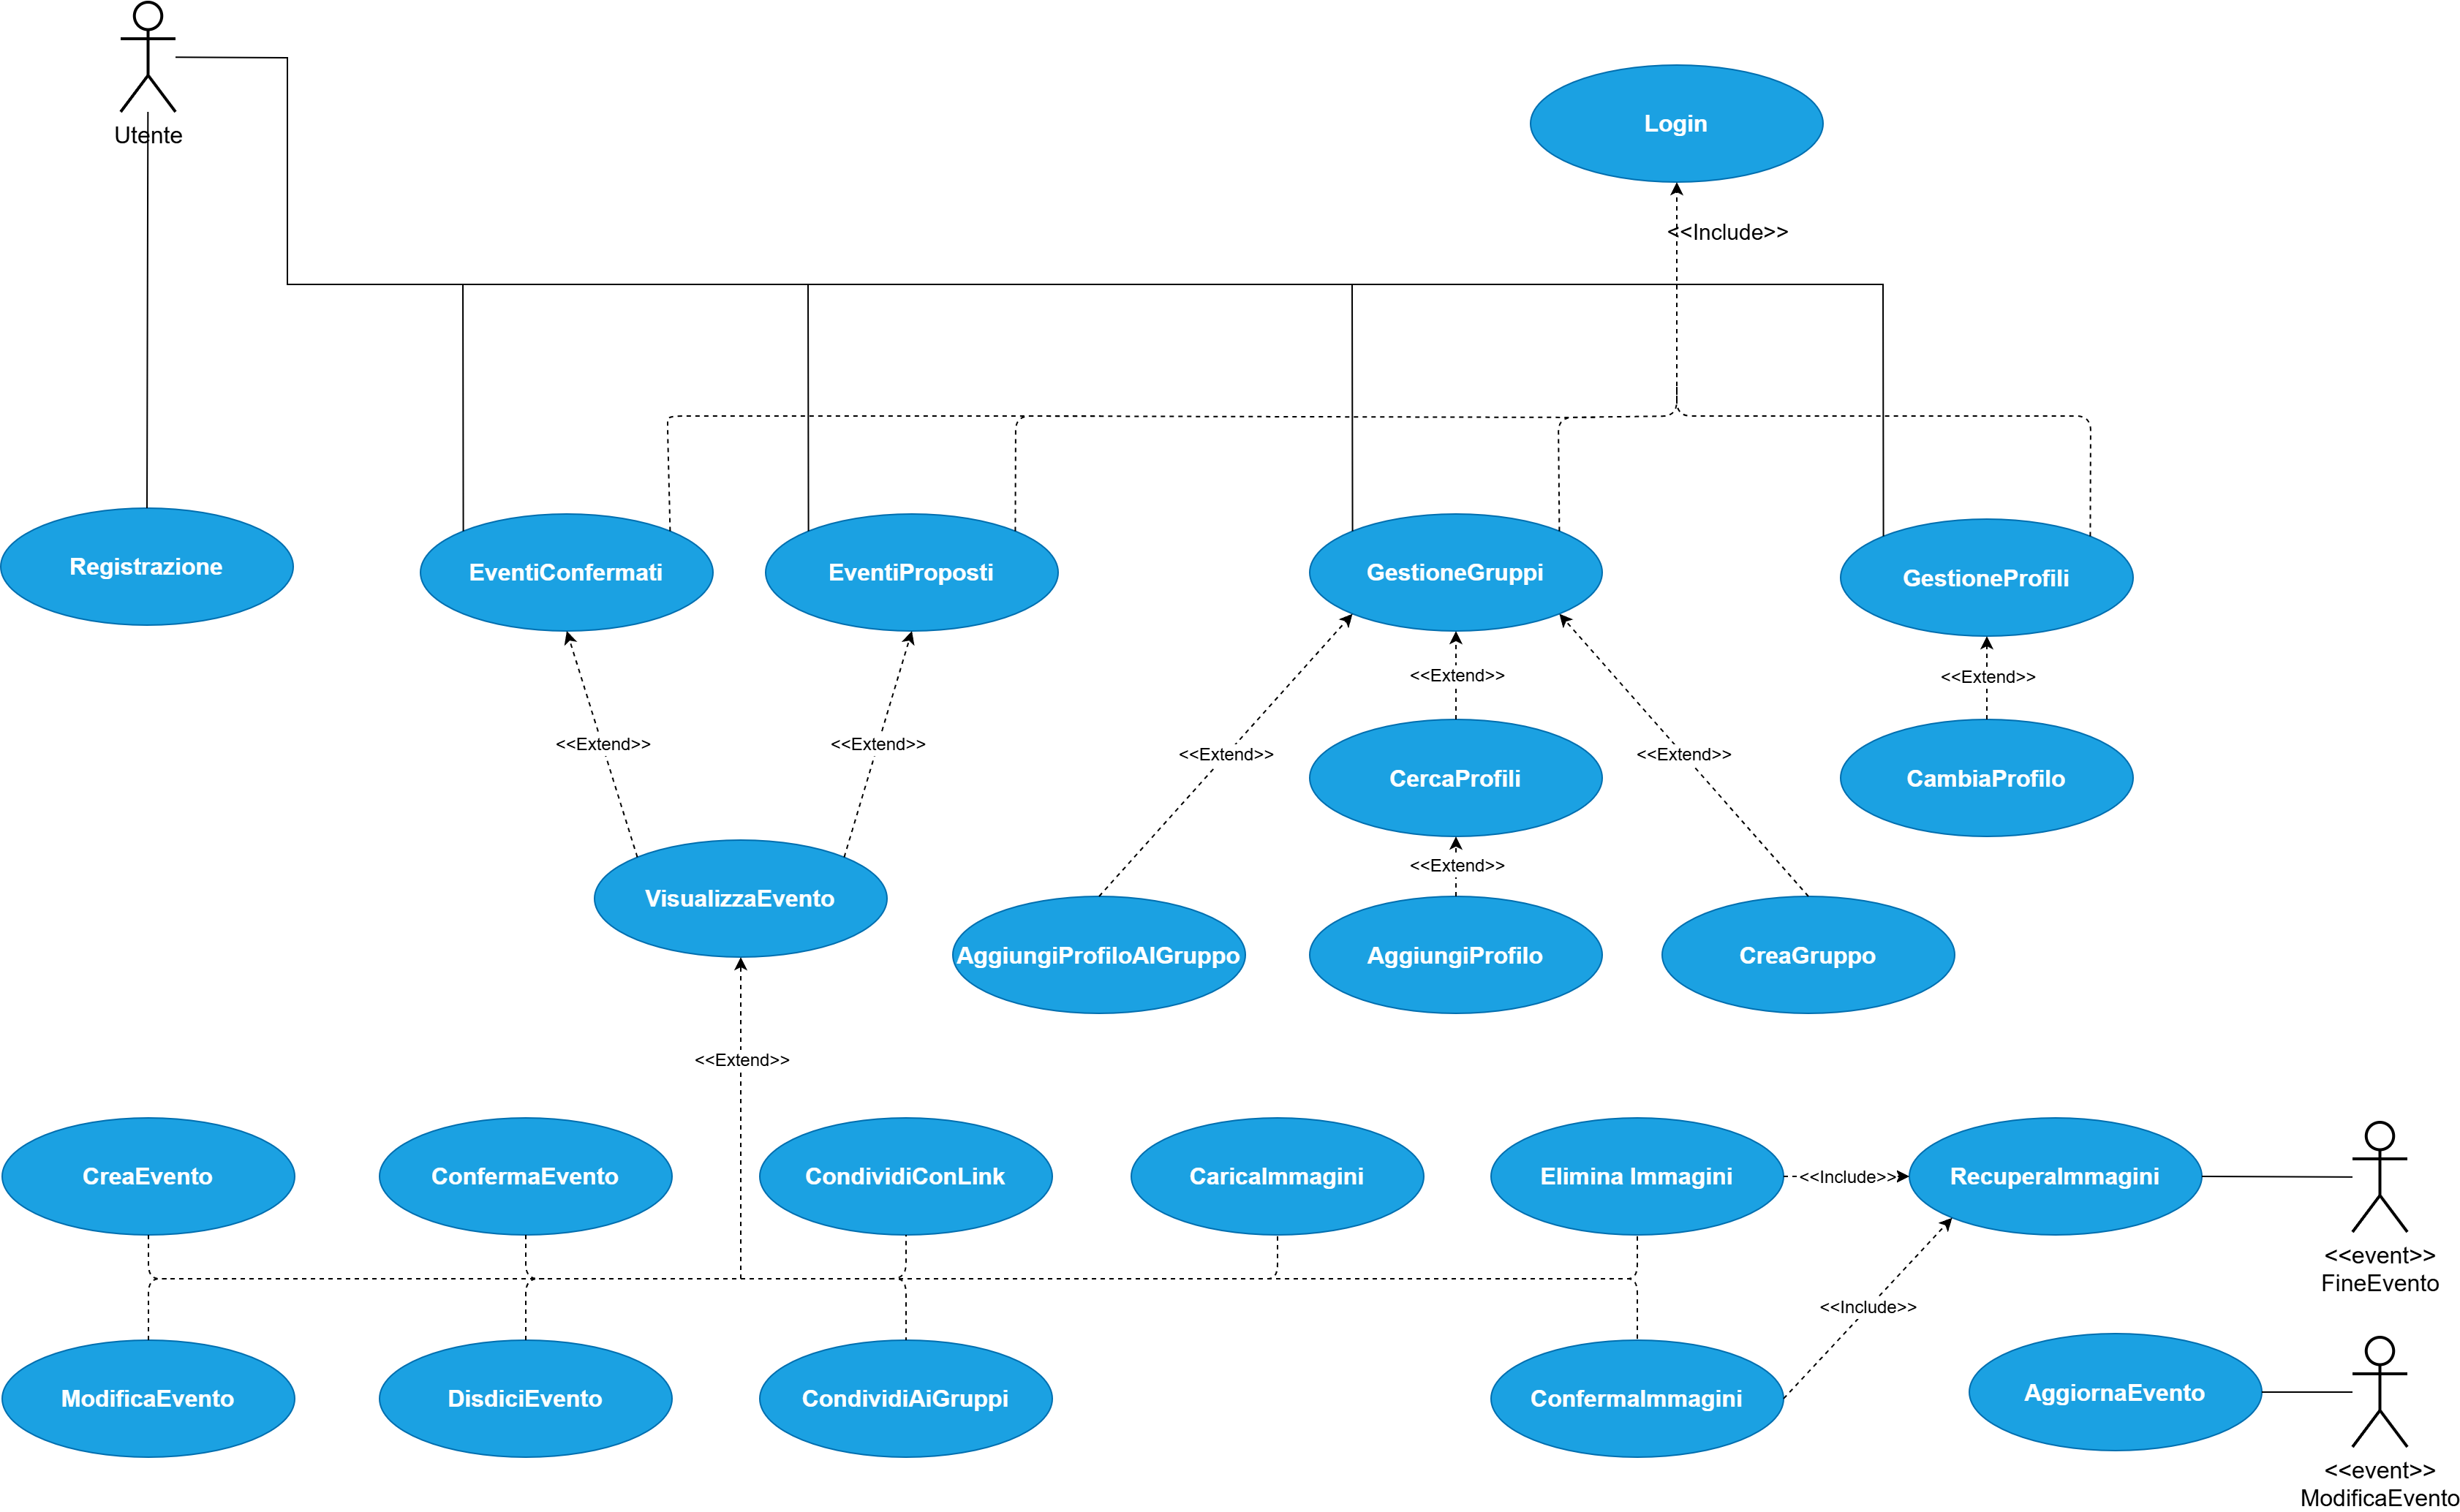
\includegraphics{Casiduso.png}}
    \caption{Diagramma dei casi d'uso}
\end{figure}

Per ogni caso d'uso viene poi identificato uno scenario di utilizzo,
che chiarifica il contesto, il comportamento e i punti critici dell'utilizzo.
Lo scenario ha il solo compito di mostrare il comportamento desiderato,
senza scendere quindi in dettagli o complessità progettuali.
Dallo scenario risulta non si può quindi dedurre la difficoltà 
introdotta dall'implementazione del caso d'uso,
ma è il tassello da cui si stabiliranno poi la coordinazione e l'interazione delle varie parti del programma.\\
\\
Si riportano gli scenari di utilizzo per i principali casi d'uso di Wyd,
ovvero quelli che più andranno a impattare sulla struttura e sulle esigenze del progetto.\\
\\
Lo scenario di registrazione vede la responsabilità, oltre che di creare un account,
di collegare un profilo all'utente.
Questa separazione consente di avere una struttura gerarchica
che permette di associare più profili a un unico utente,
che può così in seguito crearne o unirne di nuovi.\\

\begin{longtable} {|P{4.5cm}|P{11cm}|}
    \hline
    \textbf{Titolo}                   & Registrazione                                                                         \\
    \hline
    \textbf{Descrizione}              & L'utente si registra al servizio                                                      \\
    \hline
    \textbf{Attori}                   & Utente                                                                                \\
    \hline
    \textbf{Relazioni}                &                                                                                       \\
    \hline
    \textbf{Precondizioni}            &                                                                                       \\
    \hline
    \textbf{Post condizioni}          & L'utente è registrato nel sistema e può interagire con il resto dell'applicazione     \\
    \hline
    \textbf{Scenario principale}      & 1.L'utente accede alla schermata di registrazione      \newline
    2. L'utente inserisce email e  password                      \newline
    3. Il sistema crea un account con le credenziali inserite, associando un utente e un primo profilo   \newline
    4. L'utente termina la registrazione, se avvenuta con successo viene reindirizzato alla pagina principale
    \\
    \hline
    \textbf{Scenari Alternativi}      &

    Il sistema verifica che è già presente un account con la mail inserita, quindi procede con la procedura di login normale. \\
    \hline
    \textbf{Requisiti non funzionali} &
    Per interagire l'utente deve essere autenticato \newline
    Velocità in lettura e scrittura dei dati                                                                                  \\
    \hline
    \textbf{Punti aperti}             &                                                                                       \\
    \hline
    \caption{Scenario di registrazione}
\end{longtable}

A seguito della modifica di un evento,
che implica il salvataggio dei suoi nuovi dati,
viene chiesto l'aggiornamento in tempo reale verso
tutti i dispositivi di tutti gli utenti a cui l'evento è stato condiviso.
Inoltre, sarà necessario inserire un controllo per evitare
che due richieste simultanee causino conflitti.\\

\begin{longtable} {|P{4.5cm}|P{11cm}|}
    \hline
    \textbf{Titolo}                   & ModificaEvento                                                                               \\
    \hline
    \textbf{Descrizione}              & Salva le modifiche a un evento                                                               \\
    \hline
    \textbf{Attori}                   & Utente                                                                                       \\
    \hline
    \textbf{Relazioni}                & VisualizzaEvento                                                                             \\
    \hline
    \textbf{Precondizioni}            & L'evento esiste e sono stati modificati dei dati                                             \\
    \hline
    \textbf{Post condizioni}          & Le modifiche vengono salvate e propagate a tutti i profili collegati                         \\
    \hline
    \textbf{Scenario Principale}      & 1. VisualizzaEvento \newline
    2. Il sistema controlla che i dati modificati siano corretti\newline
    3. I cambiamenti vengono salvati\newline
    4. Tutti i dispositivi collegati ai profili collegati all'evento visualizzano le immagini                                        \\
    \hline
    \textbf{Scenari Alternativi}      & 2. Se i dati risultano sbagliati, il sistema notifica l'utente originario indicando l'errore \\
    \hline
    \textbf{Requisiti non funzionali} & Velocità in lettura e scrittura dei dati \newline
    Scalabilità delle richieste                                                                                                      \\
    \hline
    \textbf{Punti aperti}             & Le modifiche all'evento devono essere consistenti, \newline
    soprattutto in caso di richieste simultanee                                                                                      \\
    \hline
    \caption{Scenario della modifica di un evento}
\end{longtable}

Il salvataggio delle immagini è un'operazione di particolare importanza
vista la sua rilevanza nel coinvolgimento degli utenti
nell'utilizzo delle funzionalità centrali dell'applicazione,
e quindi nel successo del progetto.
Oltre a mostrare un'interfaccia intuitiva,
il sistema deve essere in grado di gestire queste particolari richieste di caricamento,
che generalmente necessitano di più tempo e memoria.
Prevedendo che la maggior parte di queste avvenga in seguito alla conclusione dell'evento,
la probabilità che più richieste simultanee vertano sullo stesso evento risulta elevata,
creando la necessità di una gestione parallela di modifiche concorrenti.\\

\begin{longtable} {|P{4.5cm}|P{11cm}|}
    \hline
    \textbf{Titolo}                   & CaricaImmagini                                                                  \\
    \hline
    \textbf{Descrizione}              & Permette all'utente di selezionare immagini da collegare all'evento, salvandole \\
    \hline
    \textbf{Attori}                   & Utente                                                                          \\
    \hline
    \textbf{Relazioni}                & VisualizzaEvento                                                                \\
    \hline
    \textbf{Precondizioni}            & L'evento esiste                                                                 \\
    \hline
    \textbf{Post condizioni}          & Le immagini vengono salvate e propagate a tutti i profili collegati             \\
    \hline
    \textbf{Scenario Principale}      & 1. VisualizzaEvento \newline
    2. L'utente seleziona le immagini che vuole caricare\newline
    3. Le immagini vengono salvate\newline
    4. Tutti i dispositivi relativi ai profili collegati all'evento visualizzano le immagini                            \\
    \hline
    \textbf{Scenari Alternativi}      &
    Scenario alternativo A:\newline
    3. Almeno una delle immagini crea problemi di lettura,
    l'utente viene notificato e può riprovare a caricare le immagini\newline
    Scenario alternativo B:\newline
    3. Solo una parte delle immagini vengono salvate, altre comportano errori\newline
    4. L'utente viene notificato dell'errore e può riprovare a caricare le immagini\newline
    5. Tutti i dispositivi relativi ai profili collegati all'evento visualizzano le immagini\newline
    Scenario alternativo C:\newline
    3. Nessuna immagine risulta salvata con successo\newline
    4. L'utente viene notificato dell'errore e può riprovare                                                            \\
    \hline
    \textbf{Requisiti non funzionali} & Semplicità e fluidità dell'interfaccia grafica   \newline
    Velocità in lettura e scrittura dei dati\newline
    Scalabilità delle richieste                                                                                         \\
    \hline
    \textbf{Punti aperti}             &                                                                                 \\
    \hline

    \caption{Scenario del caricamento delle immagini}
\end{longtable}

L'azione di recupero delle immagini facilita l'utilizzo dell'applicazione,
automatizzando il procedimento di ricerca delle immagini,
riducendo l'interazione utente alla sola conferma.
Una sua corretta implementazione ne fa apprezzare l'utilità,
con una significativa influenza sull'esperienza utente.
Richiede però la pianificazione e l'automazione del processo di cernita di dati,
con effetti sull'analisi tecnologica, sui processi in background e sulla gestione della memoria locale.\\

\begin{longtable} {|P{4.5cm}|P{11cm}|}
    \hline
    \textbf{Titolo}                   & RecuperaImmagini                                                                                                                           \\
    \hline
    \textbf{Descrizione}              & L'applicazione controlla la galleria e salva in locale le foto scattate durante l'evento                                                   \\
    \hline
    \textbf{Attori}                   & FineEvento                                                                                                                                 \\
    \hline
    \textbf{Relazioni}                & EliminaImmagini, ConfermaImmagini                                                                                                          \\
    \hline
    \textbf{Precondizioni}            & L'evento esiste ed è concluso\newline
    l'utente ha dato il permesso all'accesso alla galleria                                                                                                                         \\
    \hline
    \textbf{Post condizioni}          & Le immagini sono salvate in locale e l'utente viene notificato                                                                             \\
    \hline
    \textbf{Scenario Principale}      & 1. Il sistema attende la fine dell'evento\newline
    2. Il sistema controlla la galleria per trovare le immagini scattate nell'arco temporale dell'evento\newline
    3. Se ci sono immagini, vengono salvate in locale e l'utente viene notificato                                                                                                  \\
    \hline
    \textbf{Scenari Alternativi}      &                                                                                                                                            \\
    \hline
    \textbf{Requisiti non funzionali} & Velocità in lettura e scrittura dei dati                                                                                                   \\
    \hline
    \textbf{Punti aperti}             & L'implementazione dipende dal dispositivo su cui viene eseguita l'applicazione, alcuni dispositivi potrebbero non permetterne l'esecuzione \\
    \hline


    \caption{Scenario di recupero delle immagini dal dispositivo dell'utente}
\end{longtable}

\clearpage

\subsection{Requisiti di sicurezza}

Ogni sistema è esposto a vulnerabilità che impattano sul corretto funzionamento dell'applicazione
e possono comportare disservizi in base alla loro rilevanza nel funzionamento del sistema.
La rilevazione dei rischi e la successiva definizione dei requisiti necessari per evitare o minimizzare i danni
è alla base della strategia di sicurezza.\\
\\
La definizione dei requisiti di sicurezza deriva dall'analisi del rischio.
L'analisi del rischio individua i possibili vettori di attacco e serve a orientare le risorse dove più necessario,
tramite la valutazione dei beni, l'identificazione delle minacce e
l'individuazione dei punti deboli delle tecnologie di cui si prevede l'utilizzo.\\
\\
La valutazione dei beni determina i componenti fondamentali da proteggere,
risaltandone il valore e l'esposizione relativa.
Questo permette di stabilire le priorità dei componenti sui cui concentrare le attenzioni.
In particolare, Wyd non prevede altri sistemi diversi dai comuni sistemi informatici,
ma i valori principali da proteggere risiedono nei dati degli utenti.\\
\\
\begin{longtable} {|P{3.5cm}|P{5.5cm}|P{6.7cm}|}
    \hline
    \textbf{Bene}                     & \textbf{Valore}                                                                                              & \textbf{Esposizione}      \\
    \hline
    Sistema Informativo               & Alto. Fondamentale per il funzionamento del servizio                                                         &
    Alta. Perdita finanziaria e di immagine                                                                                                                                      \\
    \hline
    Informazioni dei clienti          & Alto. Informazioni personali                                                                                 &
    Alta. Perdita di immagine dovuta alla divulgazione
    di dati sensibili                                                                                                                                                            \\
    \hline
    Informazioni relativi agli eventi & Medio-alto, necessari per offrire il servizio e contenenti informazioni personali e potenzialmente riservate &
    Molto Alta. Perdita di immagine possibile con la divulgazione dei dati relativi ai
    clienti                                                                                                                                                                      \\
    \hline
    Dati dei gruppi                   & Medio. Necessario per condividere gli eventi                                                                 & Alta. Perdita di immagine \\
    \hline
    \caption{Valutazione dei beni}
\end{longtable}

\clearpage

La tabella delle minacce individua gli attacchi principali previsti che possono avvenire sul sistema.
Esamina la loro probabilità, le azioni richieste per controllarli e il costo di realizzazione delle contromisure necessarie.
Fornisce quindi una prima analisi sulle necessità implementative.\\
\\
Tutte le risorse di Wyd sono orientate agli utenti,
in particolare al mantenimento e alla distribuzione dei loro dati.
Per questo motivo le minacce sono relative alla confidenzialità dei dati o
all'interruzione del servizio.\\
\\
\begin{longtable}{|P{3.3cm}|P{1.6cm}|P{6.2cm}|P{4cm}|}
    \hline
    \textbf{Minaccia}                                                                           & \textbf{Probab.}                    & \textbf{Controllo}                                                                            & \textbf{Fattibilità}                                              \\
    \hline
    \endhead
    Furto credenziali utente                                                                    & Alta                                & Controllo sulla sicurezza della password - Log delle operazioni, autenticazione a due fattori & Costo implementativo medio                                        \\
    \hline
    Alterazione o intercettazione delle comunicazioni                                           & Alta                                & Utilizzo di un canale sicuro - Log delle operazioni, autenticazione integrata nel messaggio   & Basso costo di realizzazione con determinati protocolli           \\
    \hline
    Accesso non autorizzato al database                                                         & Bassa                               & Accesso da macchine sicure - Log di tutte le operazioni                                       & Basso costo di realizzazione, il server deve essere ben custodito \\
    \hline
    DoS                                                                                         & Bassa                               & Controllo e limitazione delle richieste                                                       & Media complessità di implementazione                              \\
    \hline
    Saturazione del database                                                                    & Bassa                               & 1. Limitazione delle richieste in un dato intervallo di tempo. \newline
    2. Limitazione della grandezza delle richieste singole \newline
    3. Limitazione della grandezza richiesta dallo stesso utente in un dato intervallo di tempo & Media complessità d'implementazione                                                                                                                                                                     \\
    \hline
    \caption{Tabella delle minacce}
\end{longtable}

\clearpage

L'analisi tecnologica della sicurezza entra nel merito 
delle tecnologie di cui si prevede l'utilizzo.
Per ognuna esamina i punti deboli e i limiti intrinseci,
producendo un quadro delle particolarità su cui porre maggiore attenzione.\\
\\
Wyd prevede principalmente la comunicazione tra le applicazioni utenti e un server centrale,
per cui la tecnologia da analizzare si concentra sull'architettura
ma soprattutto sulle comunicazioni e sull'autenticazione.\\


\begin{longtable} {|P{4cm}|P{12cm}|}
    \hline
    Tecnologia                     & Vulnerabilità                                                                         \\
    \hline
    \endhead
    Autenticazione email/password  &
    \begin{itemize}
        \item Utente rivela volontariamente la password
        \item Utente rivela la password con un attacco di ingegneria sociale
        \item Password banali
    \end{itemize}                                                    \\
    \hline
    Cifratura comunicazioni        &
    \begin{itemize}
        \item In caso di cifratura simmetrica particolare attenzione va alla lunghezza delle chiavi ed alla loro memorizzazione
    \end{itemize} \\
    \hline
    Architettura Client/Server     &
    \begin{itemize}
        \item DoS
        \item Man in the Middle
        \item Sniffing delle comunicazioni
    \end{itemize}                                                                                      \\
    \hline
    Connessione Server/Persistenza & \begin{itemize}
                                         \item Limite massimo di connessioni contemporanee
                                         \item Saturazione del Database
                                     \end{itemize}                                      \\
    \hline
    \caption{Analisi tecnologica della sicurezza}
\end{longtable}

A questo punto si prevedono i principali attori malevoli e i relativi casi d'uso,
per poi definire i requisiti su cui si baseranno le contromisure necessarie.
I casi d'uso sono molto simili alle minacce individuate in precedenza,
ma vengono creati in base alla modalità di attacco, più che alla tipologia.
A ogni caso d'uso malevolo ne viene corrisposto un altro che ne comporta la mitigazione.
Si integrano quindi con i casi d'uso dell'applicazione,
evidenziando i punti e la loro applicazione.\\
\clearpage

In Wyd sono stati individuati quattro casi d'uso malevoli,
tre dei quali relativi all'integrità e alla confidenzialità dei dati,
e uno relativo alla disponibilità del servizio.\\
\\
Tramite la saturazione del database l'attaccante
riesce a inserire quantità importanti di dati,
che può comportare un rallentamento dell'applicazione temporaneo o permanente,
in base alla configurazione dell'attacco.
Questo è particolarmente efficace dal momento in cui si possono inserire delle foto.
Per mitigare questo rischio si aggiunge un caso d'uso relativo al controllo delle dimensioni delle richieste.\\
\\
\begin{figure}[hb]
    \begin{center}
        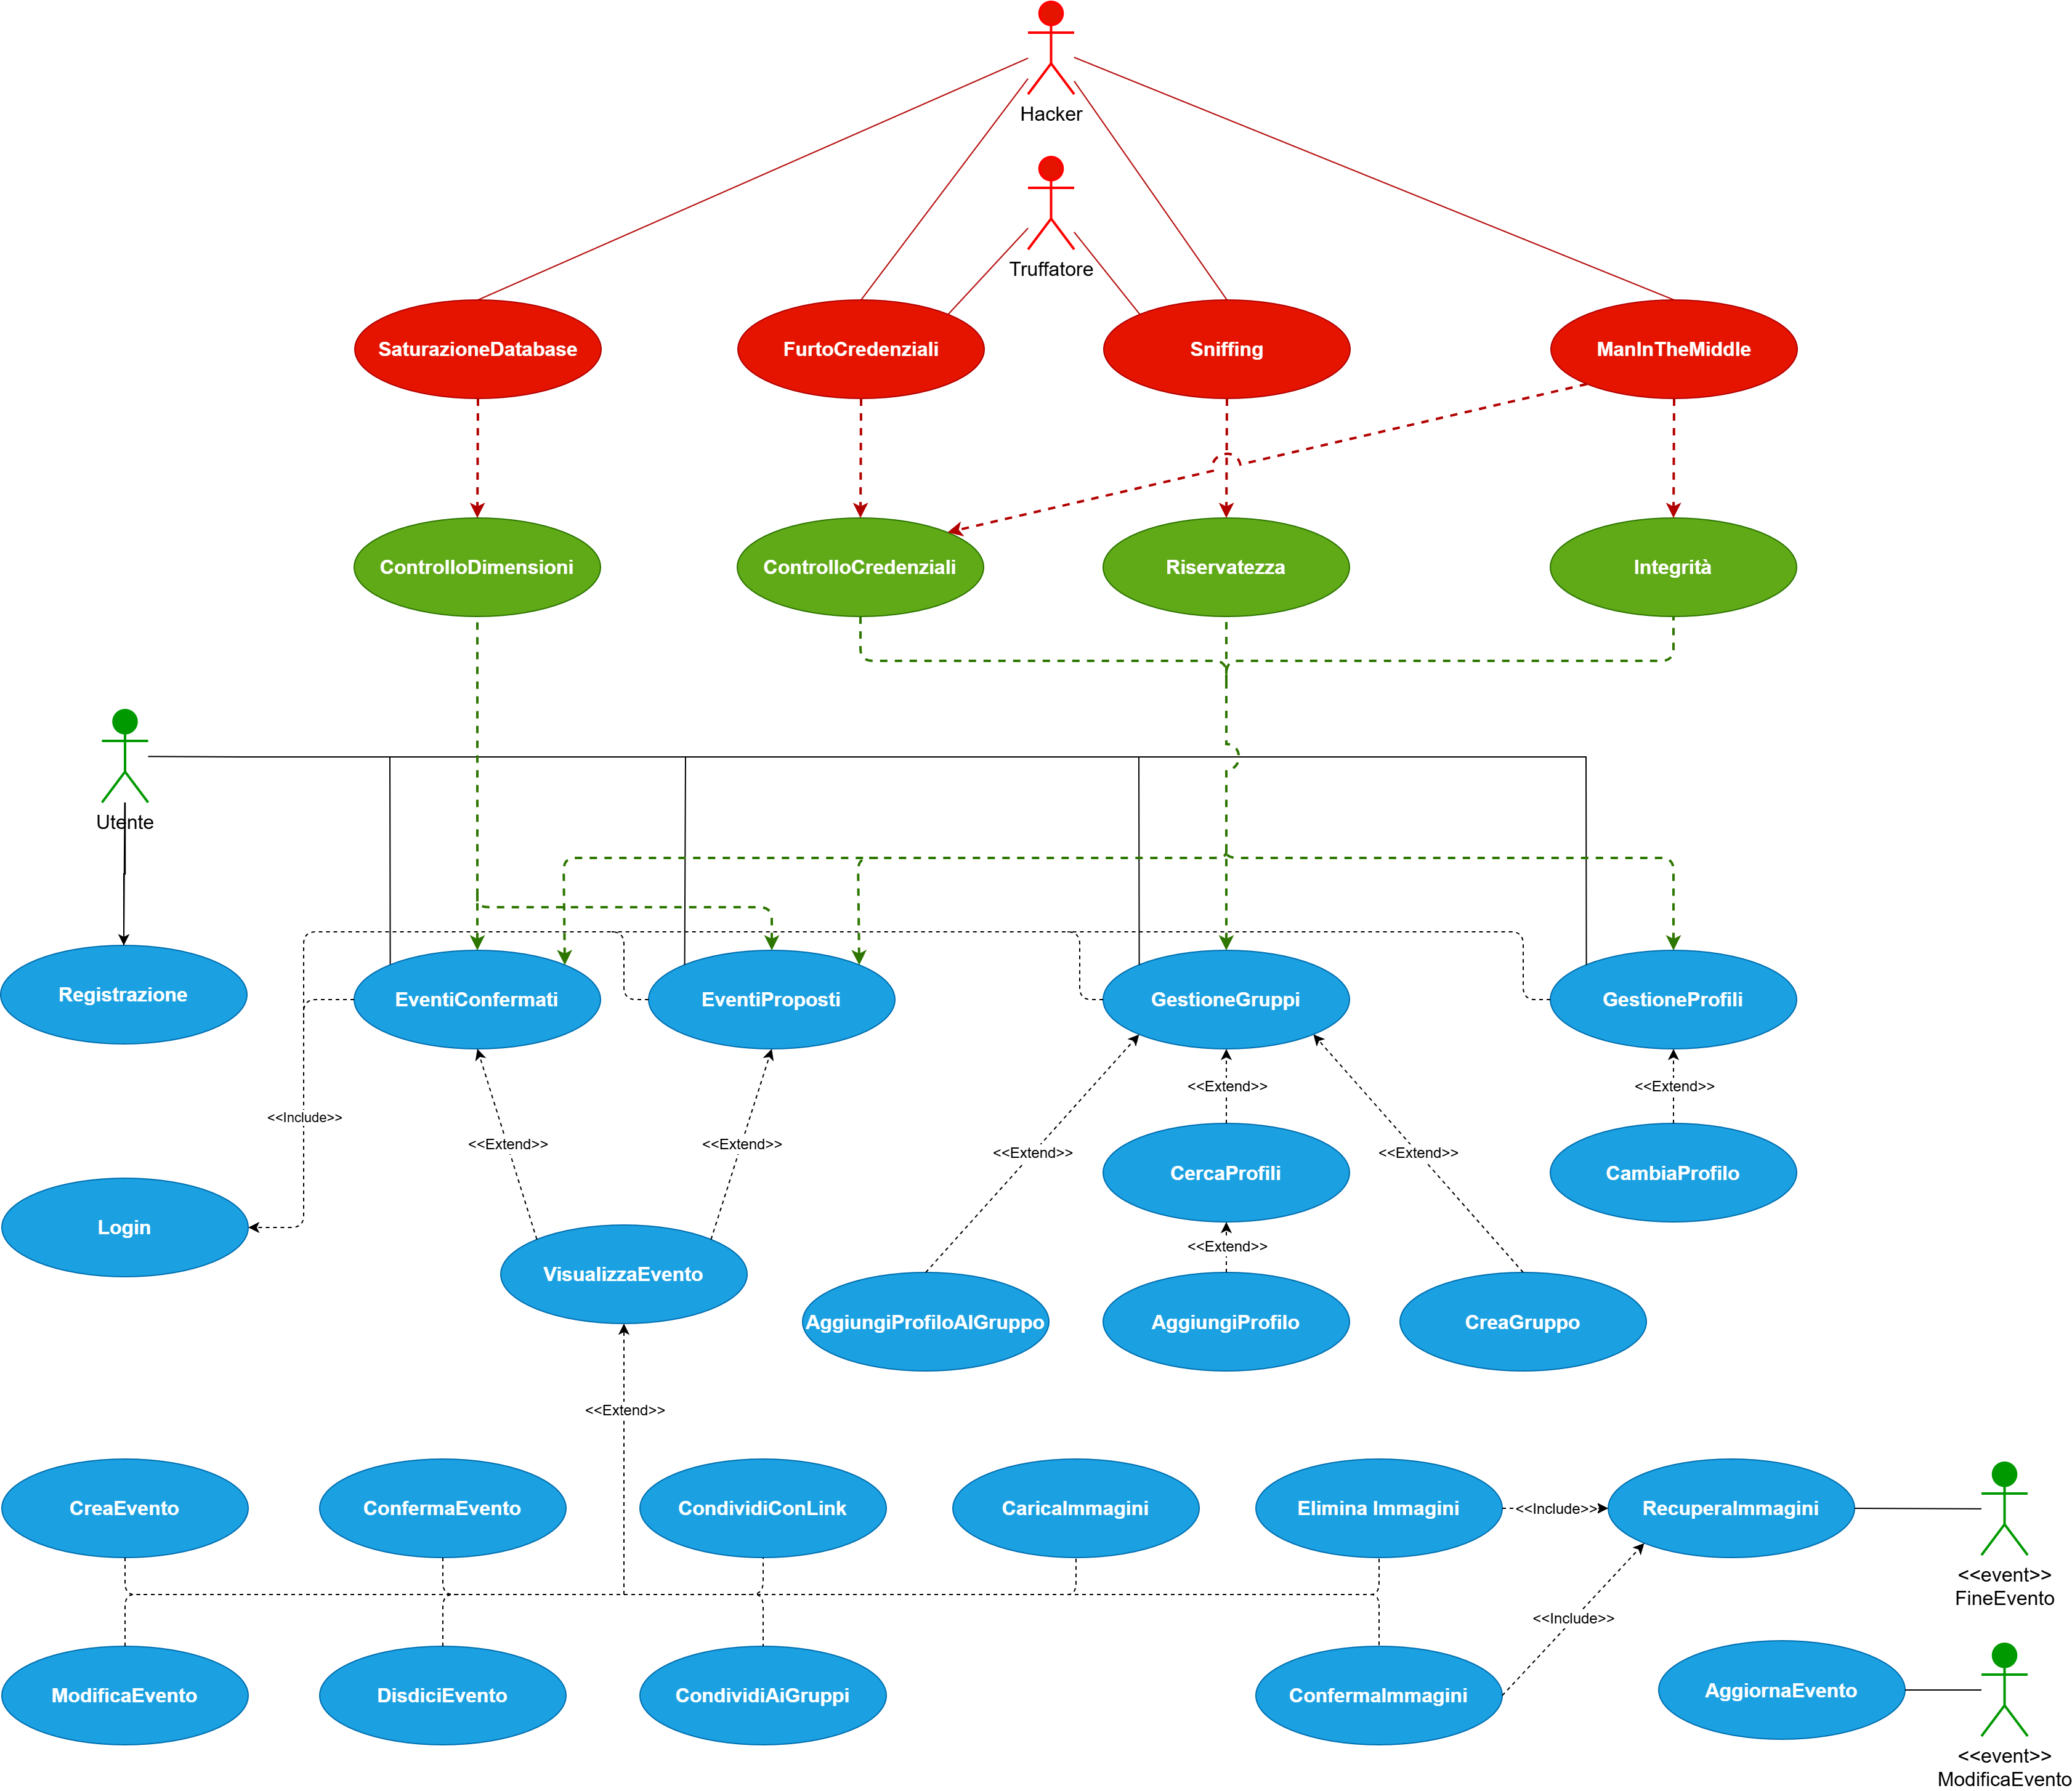
\includegraphics[height=0.6\textheight]{SecurityCase.png}
        \caption{Casi d'uso relativi alla sicurezza}
    \end{center}
\end{figure}
\clearpage

La confidenzialità e l'integrità dei dati sono minacciati dal furto di credenziali,
che permetterebbe a un utente d'identificarsi come qualcun altro;
lo sniffing mina la riservatezza delle comunicazioni, che verrebbero così intercettate;
infine tramite man in the middle un attore malevolo ha la possibilità di modificare le richieste
ingannando entrambi i lati della conversazione.
Si introducono i casi d'uso relativi al controllo delle credenziali,
che aumenta la difficoltà di un possibile furto;
la riservatezza, che permette di nascondere le comunicazioni alle parti non interessate,
e l'integrità, che consente l'individuazione di eventuale manipolazione dei messaggi.\\
\\
Visti i costi e appurate le risorse a disposizione sono stati quindi identificati i seguenti requisiti
inerenti alla protezione dei dati e delle funzionalità di Wyd:

\begin{enumerate}
    \item Implementare un sistema di log per tracciare tutti i messaggi tra i client e i server, inclusi gli accessi, le richieste di prenotazione, di conferma, di sospensione e di invio e ricezione di dati
    \item I dati salvati devono essere protetti da un attaccante che abbia accesso al sistema, prendendo misure di sicurezza fisica, eventualmente cifrando i dati
    \item I dati inviati tra le parti remote devono essere protetti, utilizzando la cifratura dei dati
    \item Tutte le azioni avvenute sul sistema devono essere tracciate tramite un sistema di log.
    \item Il sistema deve essere resistente a un alto numero di richieste contemporanee
    \item La dimensione delle richieste non deve superare una determinata soglia
\end{enumerate}

La visione e l'analisi dei log verrà gestita con uno strumento esterno,
accessibile solo al personale autorizzato.


\begin{longtable}{|P{1.3cm}|P{11.2cm}|P{3cm}|}
    \hline
    \textbf{ID}             & \textbf{Requisiti}                                                                           & \textbf{Tipo}  \\
    \hline
    \endhead
    R21F                    & Implementazione di un sistema di log per tracciare tutti i messaggi
    tra i client e i server & Funzionale                                                                                                    \\
    \hline
    R22F                    & Le richieste non devono superare una certa dimensione                                        & Funzionale     \\
    \hline
    R7NF                    & I dati salvati devono essere protetti da un attaccante che abbia
    accesso al sistema, prendendo misure di sicurezza fisica, eventualmente
    cifrando i dati         & Non Funzionale                                                                                                \\
    \hline
    R8NF                    & I dati inviati tra le parti remote devono essere protetti, utilizzando la cifratura dei dati & Non Funzionale \\
    \hline
    R9NF                    & Il sistema deve essere resistente ad un alto numero di richieste contemporanee               & Non funzionale \\
    \hline
    \caption{Requisiti di sicurezza}
\end{longtable}

\clearpage